% Options for packages loaded elsewhere
\PassOptionsToPackage{unicode}{hyperref}
\PassOptionsToPackage{hyphens}{url}
%
\documentclass[
  ignorenonframetext,
]{beamer}
\usepackage{pgfpages}
\setbeamertemplate{caption}[numbered]
\setbeamertemplate{caption label separator}{: }
\setbeamercolor{caption name}{fg=normal text.fg}
\beamertemplatenavigationsymbolsempty
% Prevent slide breaks in the middle of a paragraph
\widowpenalties 1 10000
\raggedbottom
\setbeamertemplate{part page}{
  \centering
  \begin{beamercolorbox}[sep=16pt,center]{part title}
    \usebeamerfont{part title}\insertpart\par
  \end{beamercolorbox}
}
\setbeamertemplate{section page}{
  \centering
  \begin{beamercolorbox}[sep=12pt,center]{part title}
    \usebeamerfont{section title}\insertsection\par
  \end{beamercolorbox}
}
\setbeamertemplate{subsection page}{
  \centering
  \begin{beamercolorbox}[sep=8pt,center]{part title}
    \usebeamerfont{subsection title}\insertsubsection\par
  \end{beamercolorbox}
}
\AtBeginPart{
  \frame{\partpage}
}
\AtBeginSection{
  \ifbibliography
  \else
    \frame{\sectionpage}
  \fi
}
\AtBeginSubsection{
  \frame{\subsectionpage}
}
\usepackage{lmodern}
\usepackage{amssymb,amsmath}
\usepackage{ifxetex,ifluatex}
\ifnum 0\ifxetex 1\fi\ifluatex 1\fi=0 % if pdftex
  \usepackage[T1]{fontenc}
  \usepackage[utf8]{inputenc}
  \usepackage{textcomp} % provide euro and other symbols
\else % if luatex or xetex
  \usepackage{unicode-math}
  \defaultfontfeatures{Scale=MatchLowercase}
  \defaultfontfeatures[\rmfamily]{Ligatures=TeX,Scale=1}
\fi
% Use upquote if available, for straight quotes in verbatim environments
\IfFileExists{upquote.sty}{\usepackage{upquote}}{}
\IfFileExists{microtype.sty}{% use microtype if available
  \usepackage[]{microtype}
  \UseMicrotypeSet[protrusion]{basicmath} % disable protrusion for tt fonts
}{}
\makeatletter
\@ifundefined{KOMAClassName}{% if non-KOMA class
  \IfFileExists{parskip.sty}{%
    \usepackage{parskip}
  }{% else
    \setlength{\parindent}{0pt}
    \setlength{\parskip}{6pt plus 2pt minus 1pt}}
}{% if KOMA class
  \KOMAoptions{parskip=half}}
\makeatother
\usepackage{xcolor}
\IfFileExists{xurl.sty}{\usepackage{xurl}}{} % add URL line breaks if available
\IfFileExists{bookmark.sty}{\usepackage{bookmark}}{\usepackage{hyperref}}
\hypersetup{
  pdftitle={305 Lecture 13 - Disjunction},
  pdfauthor={Brian Weatherson},
  hidelinks,
  pdfcreator={LaTeX via pandoc}}
\urlstyle{same} % disable monospaced font for URLs
\newif\ifbibliography
\usepackage{graphicx,grffile}
\makeatletter
\def\maxwidth{\ifdim\Gin@nat@width>\linewidth\linewidth\else\Gin@nat@width\fi}
\def\maxheight{\ifdim\Gin@nat@height>\textheight\textheight\else\Gin@nat@height\fi}
\makeatother
% Scale images if necessary, so that they will not overflow the page
% margins by default, and it is still possible to overwrite the defaults
% using explicit options in \includegraphics[width, height, ...]{}
\setkeys{Gin}{width=\maxwidth,height=\maxheight,keepaspectratio}
% Set default figure placement to htbp
\makeatletter
\def\fps@figure{htbp}
\makeatother
\setlength{\emergencystretch}{3em} % prevent overfull lines
\providecommand{\tightlist}{%
  \setlength{\itemsep}{0pt}\setlength{\parskip}{0pt}}
\setcounter{secnumdepth}{-\maxdimen} % remove section numbering
\let\Tiny=\tiny

 \setbeamertemplate{navigation symbols}{} 

% \usetheme{Madrid}
 \usetheme[numbering=none, progressbar=foot]{metropolis}
 \usecolortheme{wolverine}
 \usepackage{color}
 \usepackage{MnSymbol}
% \usepackage{movie15}

\usepackage{amssymb}% http://ctan.org/pkg/amssymb
\usepackage{pifont}% http://ctan.org/pkg/pifont
\newcommand{\cmark}{\ding{51}}%
\newcommand{\xmark}{\ding{55}}%

\DeclareSymbolFont{symbolsC}{U}{txsyc}{m}{n}
\DeclareMathSymbol{\boxright}{\mathrel}{symbolsC}{128}
\DeclareMathAlphabet{\mathpzc}{OT1}{pzc}{m}{it}


% \usepackage{tikz-qtree}
% \usepackage{markdown}
% \usepackage{prooftrees}
% \forestset{not line numbering, close with = x}
% Allow for easy commas inside trees
\renewcommand{\,}{\text{, }}


\usepackage{tabulary}

\usepackage{open-logic-config}

\setlength{\parskip}{1ex plus 0.5ex minus 0.2ex}

\AtBeginSection[]
{
\begin{frame}
	\Huge{\color{darkblue} \insertsection}
\end{frame}
}

\renewenvironment*{quote}	
	{\list{}{\rightmargin   \leftmargin} \item } 	
	{\endlist }

\definecolor{darkgreen}{rgb}{0,0.7,0}
\definecolor{darkblue}{rgb}{0,0,0.8}

\newcommand{\starttab}{\begin{center}
\vspace{6pt}
\begin{tabular}}

\newcommand{\stoptab}{\end{tabular}
\vspace{6pt}
\end{center}
\noindent}


\newcommand{\sif}{\rightarrow}
\newcommand{\siff}{\leftrightarrow}
\newcommand{\EF}{\end{frame}}


\newcommand{\TreeStart}[1]{
%\end{frame}
\begin{frame}
\begin{center}
\begin{tikzpicture}[scale=#1]
\tikzset{every tree node/.style={align=center,anchor=north}}
%\Tree
}

\newcommand{\TreeEnd}{
\end{tikzpicture}
%\end{center}
}

\newcommand{\DisplayArg}[2]{
\begin{enumerate}
{#1}
\end{enumerate}
\vspace{-6pt}
\hrulefill

%\hspace{14pt} #2
%{\addtolength{\leftskip}{14pt} #2}
\begin{quote}
{\normalfont #2}
\end{quote}
\vspace{12pt}
}

\newenvironment{ProofTree}[1][1]{
\begin{center}
\begin{tikzpicture}[scale=#1]
\tikzset{every tree node/.style={align=center,anchor=south}}
}
{
\end{tikzpicture}
\end{center}
}

\newcommand{\TreeFrame}[2]{
\begin{columns}[c]
\column{0.5\textwidth}
\begin{center}
\begin{prooftree}{}
#1
\end{prooftree}
\end{center}
\column{0.45\textwidth}
%\begin{markdown}
#2
%\end{markdown}
\end{columns}
}

\newcommand{\ScaledTreeFrame}[3]{
\begin{columns}[c]
\column{0.5\textwidth}
\begin{center}
\scalebox{#1}{
\begin{prooftree}{}
#2
\end{prooftree}
}
\end{center}
\column{0.45\textwidth}
%\begin{markdown}
#3
%\end{markdown}
\end{columns}
}

\usepackage[bb=boondox]{mathalfa}
\DeclareMathAlphabet{\mathbx}{U}{BOONDOX-ds}{m}{n}
\SetMathAlphabet{\mathbx}{bold}{U}{BOONDOX-ds}{b}{n}
\DeclareMathAlphabet{\mathbbx} {U}{BOONDOX-ds}{b}{n}

\RequirePackage{bussproofs}
\RequirePackage[tableaux]{prooftrees}

\newenvironment{oltableau}{\center\tableau{}} %wff format={anchor = base west}}}
       {\endtableau\endcenter}
       
\newcommand{\formula}[1]{$#1$}

\usepackage{tabulary}
\usepackage{booktabs}

\def\begincols{\begin{columns}}
\def\begincol{\begin{column}}
\def\endcol{\end{column}}
\def\endcols{\end{columns}}

\usepackage[italic]{mathastext}
\usepackage{nicefrac}

\definecolor{mygreen}{RGB}{0, 100, 0}
\definecolor{mypink2}{RGB}{219, 48, 122}
\definecolor{dodgerblue}{RGB}{30,144,255}

\def\True{\textcolor{dodgerblue}{\text{T}}}
\def\False{\textcolor{red}{\text{F}}}

\title{305 Lecture 13 - Disjunction}
\author{Brian Weatherson}
\date{July 8, 2020}

\begin{document}
\frame{\titlepage}

\begin{frame}{Plan for Today}
\protect\hypertarget{plan-for-today}{}

\begin{itemize}
\tightlist
\item
  We're going to talk about how `or' behaves in Carnap.
\item
  Sentences with `or' as the main connective are called
  \textbf{disjunctions}, and the parts either side of the `or' are
  called disjuncts.
\end{itemize}

\end{frame}

\begin{frame}{Associated Reading}
\protect\hypertarget{associated-reading}{}

Carnap book, chapter 8, section ``Modus Tollendo Ponens and Addition''
(about 1/2 way down).

\end{frame}

\begin{frame}{Two Rules for Or}
\protect\hypertarget{two-rules-for-or}{}

\begin{itemize}
\tightlist
\item
  Like with `and', there is a rule for proving an `or' sentence, and a
  rule for using an `or' sentence.
\item
  The first is easy; the second is not so easy.
\end{itemize}

\end{frame}

\begin{frame}{Proving a Disjunction}
\protect\hypertarget{proving-a-disjunction}{}

\begin{itemize}
\tightlist
\item
  If you have \(A\), or for that matter if you have \(B\), you can infer
  \(A \vee B\).
\item
  The rule is called `Addition', and abbreviated `ADD'.
\item
  You cite the line that \(A\) (or \(B\), if you are doing
  `left-addition') appears on.
\end{itemize}

\end{frame}

\begin{frame}{Using a Disjunction}
\protect\hypertarget{using-a-disjunction}{}

The idea here is to take the following argument as a basic valid
argument.

\begin{quote}
\(P \vee Q, \neg Q \vdash P\)
\end{quote}

This is sometimes called \textbf{disjunctive syllogism}.

\end{frame}

\begin{frame}{Example}
\protect\hypertarget{example}{}

\begin{enumerate}
\tightlist
\item
  Either the butler did it or the gardener did it.
\item
  The gardener didn't do it.
\item
  So, the butler did it.
\end{enumerate}

\end{frame}

\begin{frame}{Another Example}
\protect\hypertarget{another-example}{}

\begin{enumerate}
\tightlist
\item
  The cat raced down the left alley or the right alley.
\item
  The cat did not race down the right alley.
\item
  So, the cat raced down the left alley.
\end{enumerate}

\end{frame}

\begin{frame}{Both Directions}
\protect\hypertarget{both-directions}{}

This looks just as plausible a bit of reasoning.

\begin{enumerate}
\tightlist
\item
  Either the butler did it or the gardener did it.
\item
  The butler didn't do it.
\item
  So, the gardener did it.
\end{enumerate}

It doesn't seem like whether we negate the first or second disjunct
matters.

\end{frame}

\begin{frame}{The Rule (first version)}
\protect\hypertarget{the-rule-first-version}{}

\begin{itemize}
\tightlist
\item
  Given \(A \vee B\) and \(\neg B\), we can infer \(A\).
\item
  The rule has a Latin name and abbreviated `MTP'. (I'm just calling it
  disjunctive syllogism.)
\item
  You cite the lines where \(A \vee B\) and \(\neg B\) appear.
\end{itemize}

\end{frame}

\begin{frame}{The Rule (second version)}
\protect\hypertarget{the-rule-second-version}{}

\begin{itemize}
\tightlist
\item
  Given \(A \vee B\) and \(\neg A\), we can infer \(B\).
\item
  The rule has a Latin name and abbreviated `MTP'. (I'm just calling it
  disjunctive syllogism.)
\item
  You cite the lines where \(A \vee B\) and \(\neg A\) appear.
\end{itemize}

\end{frame}

\begin{frame}{Caveat}
\protect\hypertarget{caveat}{}

\begin{itemize}
\tightlist
\item
  You must have the `positive' form in the disjunction and the negative
  form on a separate line.
\item
  So the argument on the next slide will not be marked as correct by
  Carnap.
\end{itemize}

\end{frame}

\begin{frame}[fragile]{Bad Use of Disjunctive Syllogism}
\protect\hypertarget{bad-use-of-disjunctive-syllogism}{}

\begin{verbatim}
6. P \/ ~Q
7. Q
8. P         :MTP 6, 7
\end{verbatim}

\end{frame}

\begin{frame}[fragile]{Correct Use of Disjunctive Syllogism}
\protect\hypertarget{correct-use-of-disjunctive-syllogism}{}

\begin{verbatim}
6. P \/ ~Q
7. Q
8. ~~Q       :DNI 7
9. P         :MTP 6, 8
\end{verbatim}

\end{frame}

\begin{frame}{A Core Argument}
\protect\hypertarget{a-core-argument}{}

The following two claims look like they should be equivalent.

\begin{enumerate}
\tightlist
\item
  \((P \vee Q) \rightarrow R\)
\item
  \((P \rightarrow R) \wedge (Q \rightarrow R)\)
\end{enumerate}

Substitute some real sentences for \(P, Q, R\) to see if this sounds
right.

\end{frame}

\begin{frame}{Exercise}
\protect\hypertarget{exercise}{}

Prove each of these

\begin{quote}
\((P \vee Q) \rightarrow R \vdash (P \rightarrow R) \wedge (Q \rightarrow R)\)
\((P \rightarrow R) \wedge (Q \rightarrow R) \vdash (P \vee Q) \rightarrow R\)
\end{quote}

\end{frame}

\begin{frame}{First One}
\protect\hypertarget{first-one}{}

\begin{figure}
\centering
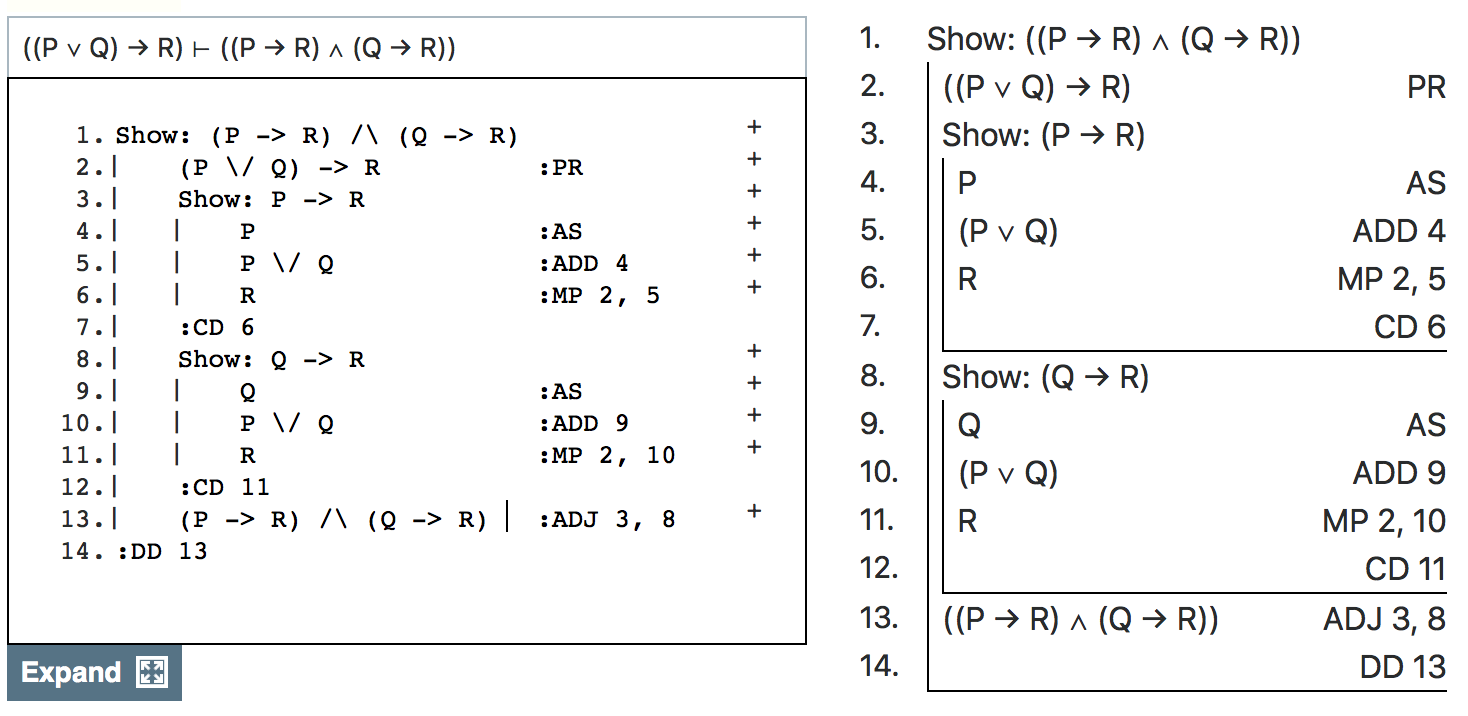
\includegraphics{../images/class05/Class-05-1.png}
\caption{\((P \vee Q) \rightarrow R \vdash (P \rightarrow R) \wedge (Q \rightarrow R)\)}
\end{figure}

\end{frame}

\begin{frame}[fragile]{Text Version of Proof}
\protect\hypertarget{text-version-of-proof}{}

\begin{verbatim}
1.  Show: (P -> R) /\ (Q -> R)
2.      (P \/ Q) -> R          :PR
3.     Show: P -> R
4.         P                  :AS
5.         P \/ Q             :ADD 4
6.         R                  :MP 2, 5
7.     :CD 6
8.     Show: Q -> R
9.         Q                  :AS
10.        P \/ Q             :ADD 9
11.        R                  :MP 2, 10
12.    :CD 11
13.    (P -> R) /\ (Q -> R)   :ADJ 3, 8
14. :DD 13
\end{verbatim}

\end{frame}

\begin{frame}{Reverse Direction}
\protect\hypertarget{reverse-direction}{}

\begin{figure}
\centering
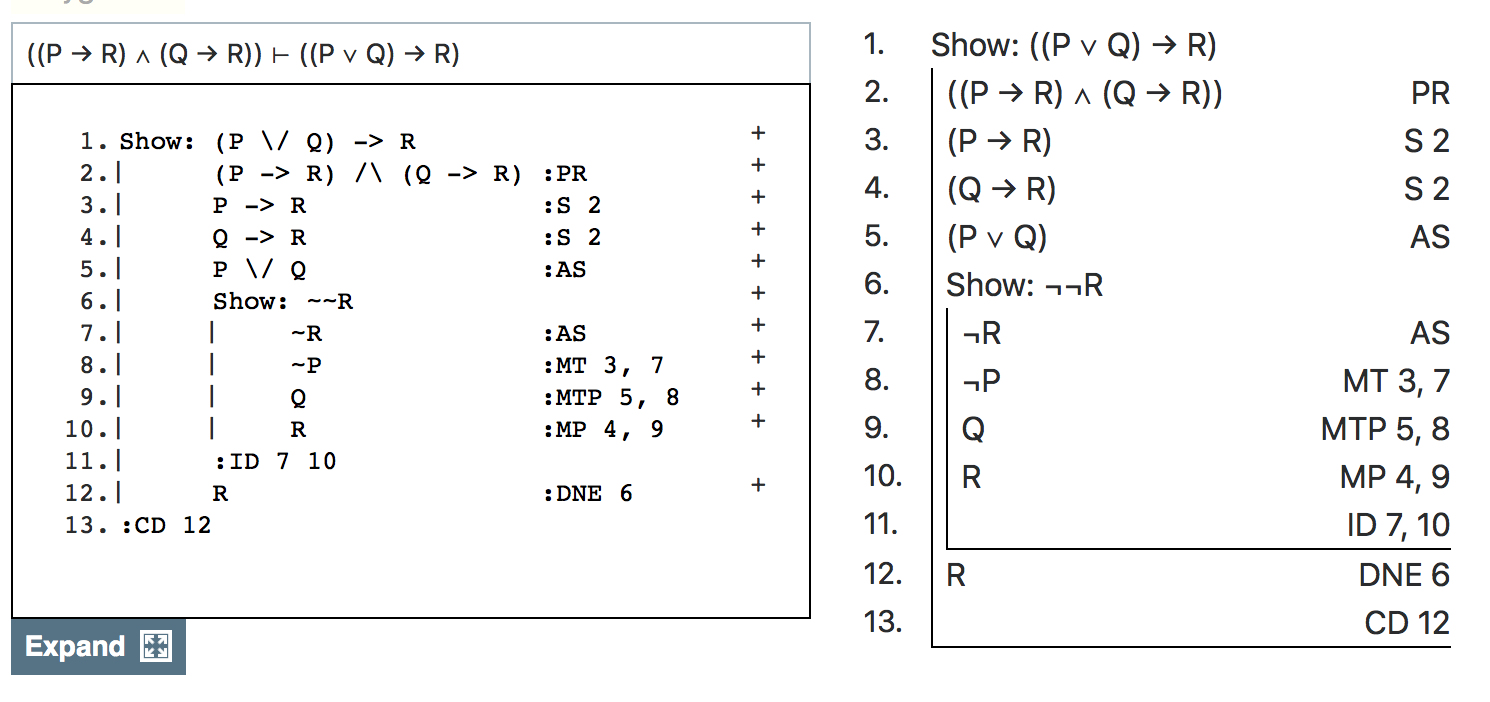
\includegraphics{../images/class05/Class-05-2.png}
\caption{\((P \rightarrow R) \wedge (Q \rightarrow R) \vdash (P \vee Q) \rightarrow R\)}
\end{figure}

\end{frame}

\begin{frame}[fragile]{Text Version of Proof}
\protect\hypertarget{text-version-of-proof-1}{}

\begin{verbatim}
1. Show: (P \/ Q) -> R
2.       (P -> R) /\ (Q -> R) :PR
3.       P -> R               :S 2
4.       Q -> R               :S 2
5.       P \/ Q               :AS
6.       Show: ~~R
7.            ~R              :AS
8.            ~P              :MT 3, 7
9.            Q               :MTP 5, 8
10.           R               :MP 4, 9
11.      :ID 7 10
12.      R                    :DNE 6
13. :CD 12
\end{verbatim}

\end{frame}

\begin{frame}{For Next Time}
\protect\hypertarget{for-next-time}{}

We'll talk about how `and' and `or' interact.

\end{frame}

\end{document}
